\documentclass{sig-alternate}
\usepackage{epsfig}
\usepackage{algorithm}
\usepackage{algorithmic}

\title{Partitioning a Structured Stream Graph \\ Using Dynamic Programming}
\numberofauthors{1}
\author{
\alignauthor \vspace{-18pt}
William Thies,
Jasper Lin, and
Saman Amarasinghe \\
	\vspace{8pt}
	\{thies, jasperln, saman\}@lcs.mit.edu \\
	\vspace{8pt}
	Laboratory for Computer Science \\
	Massachusetts Institute of Technology}

\begin{document}

  \newtheorem{definition}{Definition}
  \newtheorem{transformation}{Transformation}
  
  \maketitle
  
  \newcommand{\mt}[1]{\mbox{\it #1}}
  \newcommand{\todo}[1]{\framebox{\bf #1}}
  
  \begin{abstract}
    Applications that are structured around some notion of a "stream"
are becoming increasingly important and widespread.  There is
evidence that streaming media applications are already consuming
most of the cycles on consumer machines \cite{Rix98}, and their
use is continuing to grow.  {\StreamIt} is a language and compiler
specifically designed for modern stream programming.  Despite the
prevalence of these applications, there is surprisingly little
language and compiler for practical, large-scale stream
programming.  {\StreamIt} is a language and compiler specifically
designed for modern stream programming.  The {\StreamIt} langauge
holds two goals: first, to provide high-level stream abstractions
that improve programmer productivity and program robustness within
the streaming domain; second, to serve as a common machine
language for grid-based processors.  At the same time, {\StreamIt}
compiler aims to perform stream-specific optimizations to achieve
the performance of an expert programmer.  This thesis develops
several techniques for scheduling execution of {\filters} in
{\StreamIt}.  The work focuses on correctness as well as
minimizing buffering requirements and stored schedule size.

  \end{abstract}

  \section{Introduction}

The domain of stream programs is important because it stands at the
intersection of trends in applications and architectures.  Stream
programming naturally represents applications such as audio, video,
digital signal processing, and data analysis; applications that are
increasing prevalent as computing moves towards data-centric
applications and to the mobile and embedded space.  Also, by virtue of
their structure -- a graph of independent computational nodes (termed
{\it filters}) with explicit and regular communication -- stream
programs are a natural fit for exploiting coarse-grained parallelism
suitable for multicore architectures.  The interest in streaming
applications has spawned a number of streaming languages that target
the streaming domain, including StreamIt~\cite{streamitcc},
Brook~\cite{brook04}, Cg~\cite{cg03},
SPUR~\cite{spur05samos}, Spidle~\cite{spidle03}, Lime~\cite{lime10},
and SPL~\cite{spl09}.

In a stream program, filters define an atomic execution step that
repeats for many iterations; each execution step discards a number of
data items from filter's input edge.  Often, a filter does not discard
all the data items that it read for the current execution step,
requiring these inspected (but not discarded) items for a future
iteration (or iterations) of the filter.  This type of filter is
described as performing a sliding window computation on its
input. Sliding window computations are prevalent in stream programs.
Examples of sliding window computations include FIR filters; moving
averages and differences; error correcting codes; motion estimation;
and network packet inspection.  A recent study of a large streaming
benchmark suite written in the StreamIt programming language finds
that 17 of the 30 real-world benchmarks include at least one filter
that performs a sliding window computation~\cite{streamit-suite}.


Figure~\ref{fig:fir-nopeeking} shows how to perform a sliding
window FIR filter via state carried between iterations of a filter.
This implementation is difficult for the compiler to analyze and
reason about.  Some programming languages (e.g., Brook, Lime,
StreamIt, and IBM SPL) go so far as to include idioms that directly
represent sliding window computation, allowing the programmer to
specify, for each filter, the size of the window and the number of
items discarded after an execution of the filter.
Figure~\ref{fig:fir-peeking} shows how language extensions of the
StreamIt programming language elegantly expose sliding windows for
compiler analysis and optimization.

A goal of stream programming is to directly expose to the software
layer the necessary information to enable automatic management of
coarse-grained parallelism.  Stream programs expose multiple forms of
parallelism: pipeline parallelism that exists between producers and
consumers; task parallelism that exists between pairs of filters on
parallel branches of the stream graph; and data parallelism that
exists when a filter is stateless and can thus be replicated.  Data
parallelism is the most attractive, as it provides load-balanced and
limitless parallelism (as long as input data is available).  A filter
that is stateful, and cannot be data-parallelized, becomes a limit to
parallelization scalability, as the work of that filter cannot be
divided; the most load-intensive stateful filter becomes a
bottleneck.

This paper presents a compiler framework for data-parallelizing
filters that perform sliding window computations when the properties
of the sliding window can be calculated statically.  If sliding window
filters required state, this state would represent a new
parallelization bottleneck.  Sliding windows are the bottleneck in 11
of the 17 real-world benchmarks in the StreamIt Benchmark Suite that
contain sliding windows~\cite{streamit-suite}.  For example, examining
the Channelvocoder benchmark, this state would limit scalability to 18
cores, whereas our techniques scale to at least 64 cores.

Data-parallelizing a filter is performed via a transformation termed
{\it fission} (verb form {\it fiss})~\cite{streamit-asplos}.  Fission
is the process of data-parallelizing a stateless filter by duplicating
the filter a certain number of ways, assigning duplicates to distinct
cores, and correctly distributed input data to and collecting output
data from the duplicates.  The duplicated filters are referred to as
{\it products}.  When a sliding window is present, fission is
accomplished by duplicating certain input items since they are
required by multiple products.  This duplication translates into
inter-core communication, a limiting factor for scalability when
targeting multicore architectures.

Previous approaches duplicate each input data item to all products,
with products ignoring (decimating) items that are not
needed~\cite{streamit-asplos}.  We will show that this strategy limits
scalability for multicores by requiring too much inter-core
communication.  In contrast, our strategy precisely routes each input
item to the minimal set of product filters that requires the item.
Unlike previous work, our techniques are defined on
multiple input and multiple output filters, removing the need to
introduce synchronization filters that serialize data before and
after the product filters.  

Our techniques operate on {\it static-rate} stream graphs, meaning
that the number of items produced, the number of items consumed, and
the number of items inspected by each filter can be determined
statically.  Because of this property, a steady-state schedule of
filter firings can be calculated that does not grow buffers and can be
executed indefinitely~\cite{lee87}.  Our techniques are conscious of
the spatial locality between producers and consumers.  Our framework
includes techniques that can determine when spatial locality can be
increased by altering the steady-state schedule.  When applicable, our
techniques can reduce the overall sharing (and thus inter-core
communication) requirement to below a threshold percent of the total
input communication for each sliding window filter that is
data-parallelized. 

\begin{figure}[t]
\centering
\subfigure[]{\includegraphics[width=3.3in]{figures/fir-nopeeking.pdf}\label{fig:fir-nopeeking}}
\subfigure[]{\includegraphics[width=3.3in]{figures/fir-peeking.pdf}\label{fig:fir-peeking}}
\caption[Two implementations of an FIR filter.]{\label{fig:fir-code}
  Two StreamIt implementations of an FIR filter:
   (a) the non-peeking version implemented via a
  stateful circular buffer; and (b) the peeking version. Only steady-state implementation is
  given.}
\end{figure}

The framework presented is defined on a model of computation that is
agnostic of source language.  To evaluate our techniques we have
implemented them in the context of the StreamIt compiler
infrastructure~\cite{gordon-asplos06}.  Our transformations are guided
by the parallelization management techniques presented
in~\cite{gordon-asplos06}.  We employ 3 real-world benchmarks from the
StreamIt Benchmark Suite~\cite{streamit-suite} that include sliding
window computation.  We demonstrate the effectiveness of our
techniques by comparing them to previously published techniques on 2
multicore architectures: a 16-core SMP shared-memory multicore and the
64-core distributed-memory Tilera TILE64.  We show that
our techniques are required to achieve scalable parallelization on
both architectures, achieving a 6.7x mean speedup on the 16-core SMP
and a 1.8x mean speedup on the 64-core distributed memory multicore
over a previously published technique.

\subsection{Contributions}
This paper makes the following contributions:
\begin{itemize}
  % \myitem{Motivation for Exposing Sliding Windows in Stream
  %   Languages}: Without exposing sliding windows in the language, it
  % requires heroic effort by the compiler to analyze the access patterns
  % of such a filter. Without success, the compiler will not be able to
  % data-parallelize these filters.  This will prevent robust 
  % parallelization scalability for streaming applications.

  \myitem{Generalized Fission of Sliding Window Filters}: We present a
  transformation that fisses sliding window filters with multiple
  input and multiple outputs.  The technique also supports filters
  that with multiple schedules of execution.  General fission defines
  a precise pattern of communication of input data to the products
  that can be reasoned upon by our other techniques.

  \myitem{Sharing Reduction}: We are the first to present a technique
  that decides when it is possible to decrease the amount of sharing
  between fission products by altering the steady-state of a stream
  graph, thus decreasing inter-core communication.  The technique
  reasons about all the sliding window filters of the stream graph,
  and when possible, reduces the sharing requirement to below a given
  threshold percent of the total input of the filters. 

  \myitem{Data Parallelization of Stream Graph}: We present a
  framework for data-parallelizing all of the filters of a stream
  graph employing the fission transformation on individual filters and
  applying sharing reduction when possible.  This framework optimizes
  for spatial locality and enables the compiler to automatically and
  effectively manage parallelization across varying multicore
  architectures.

  \myitem{Enable Robust Parallelization Scaling for Multicores}: For
  streaming applications with sliding window computation, previously
  published data-parallelization transformations do not scale for our
  target multicores. Our techniques enable robust parallelization
  scalability by reducing inter-core communication.  We achieve a 17x
  mean parallelization speedup for a 16-core SMP and a 62.3x mean
  parallelization speedup for the 64-core TILE64 across our benchmarks.

\end{itemize}

% \begin{figure}[t]
% \centering
% \begin{subfloat}
% \begin{minipage}[b]{0.45\textwidth}
% \eightpoint
% \begin{verbatim}
% float->float filter FIR(int N) {
%   int srcBuffer[N];
%   int srcEnd = 0; 
%   ...
%   work push 1 pop 1 {
%     srcBuffer[srcEnd] = pop();
%     float sum = 0;
%     for (int i=0; i<N; i++) {
%       sum += weights[i] * srcBuffer[(srcEnd + i + 1) % N];
%     }
%     push(sum);
%     srcEnd = (srcEnd + 1) % N;
%   }
% }
% \end{verbatim}
% \vspace{-8pt}
% \end{minipage}%
% \caption{ \label{fig:fir-nopeeking}}
% \end{subfloat}%
% \qquad
% \begin{subfloat}
% \begin{minipage}[b]{0.45\textwidth}
% \eightpoint
% \begin{verbatim}
% float->float filter FIR(int N) {
%   ...
%   work push 1 pop 1 peek N {
%     float sum = 0;
%     for (int i=0; i<N; i++) {
%       sum += weights[i] * peek(i);
%     }
%     push(sum);
%     pop();
%   }
% }
% \end{verbatim}
% \vspace{-18pt}
% \end{minipage}
% \caption{ \label{fig:fir-streamit}}
% \end{subfloat}
% \caption[Two implementations of an FIR filter.]{\label{fig:fir-code}
%   Two StreamIt implementations of an FIR filter:
%    \subref{fig:fir-nopeeking} the non-peeking version implemented via a
%   stateful circular buffer; and \subref{fig:fir-streamit} the peeking version. Only steady-state implementation is
%   given.}
% \end{figure}

  \Section{StreamIt Programming Language}
\label{sec:streamit}

StreamIt~\cite{streamit-cc} is an architecture independent language
that is designed for stream programming. In StreamIt, programs are
represented as graphs where nodes represent computation and edges
represent FIFO-ordered communication of data over tapes. The language
features several novelties that are essential for large scale program
development. The language is modular, parameterizable, malleable and
architecture independent. In addition, the language exposes the
inherent parallelism and communication patterns that are prevalent in
streaming programs.

\begin{figure*}[t]
  \begin{minipage}[t]{4.0in}
    {
	\begin{scriptsize}
	  \begin{verbatim}
	    int->int filter ZigZagScan(int N, int[N] Order)
	    {
	        work pop N push N {
	        for (int i = 0; i < N; i++) {
	          int pixel = peek(Order[i]);
	          push(pixel);
	        }
	        for (int i = 0; i < N; i++) {
	          pop();
	        }
	      }
	    }
	  \end{verbatim}
	\end{scriptsize}
    }
    % \vspace{-3pt}
    \caption{Example filter implementing zig-zag scanning.}
    % \label{fig:zigzag-filter}
  \end{minipage}
  ~~\vrule~~
  \begin{minipage}[t]{3.0in}
    {  
	\begin{scriptsize}
	  \begin{verbatim}
	    int[64] Ordering = 
	      {00, 01, 05, 06, 14, 15, 27, 28,
	       02, 04, 07, 13, 16, 26, 29, 42,
	       03, 08, 12, 17, 25, 30, 41, 43,
	       09, 11, 18, 24, 31, 40, 44, 53,
	       10, 19, 23, 32, 39, 45, 52, 54,
	       20, 22, 33, 38, 46, 51, 55, 60,
	       21, 34, 37, 47, 50, 56, 59, 61,
	       35, 36, 48, 49, 57, 58, 62, 63};



	  \end{verbatim}
	\end{scriptsize}
    }
    % \vspace{-3pt}
    \caption{Example zig-zag order for filter.}
    \label{fig:zigzag-order}
  \end{minipage}
\end{figure*}

\SubSection{Filters as Programmable Units}
In StreamIt, the basic programmable unit is a {\it filter}. Each
filter contains a work function that executes atomically, popping
(i.e., reading) a fixed number of items from the filter input tape
and pushing (i.e., writing) a fixed number of items to the filter
output tape. A filter may also {\tt peek} at a given index on its
input tape without consuming the item; this makes it simple to
represent computation over a sliding window or performing permutations
on the input stream. The {\tt push}, {\tt pop}, and {\tt peek} rates
are declared as part of the work function, thereby enabling the
compiler to apply various optimizations and construct efficient
execution schedules. 

A filter is akin to a class in object oriented programming with the
work function serving as the main method. A filter is parameterizable,
and this allows for greater malleability and code reuse. An example
filter is shown in Figure~\ref{fig:zigzag-filter}. This filter
consumes a stream whose elements are of type {\tt int} and produces a
stream of the same type. It implements the zig-zag scanning pattern
used in the run-length encoding of quantized DCT coefficients (see
Figure~\ref{fig:zigzag}). Typically, the zig-zag scan operates on a
8x8 matrix. An instantiation of a filter can specify the matrix
dimensions, as well as the desired ordering. In MPEG, there are two
possible scan orders. The {\tt Order} parameter can define the
specific scan pattern that is desired. For example, to implement the
order shown in Figure~\ref{fig:zigzag}(a), the array is defined as
shown in Figure~\ref{fig:zigzag-order}.

In this example, the DCT matrix is represented as a unidimensional
stream. The filter peeks or inspects the elements and copies them to
the output stream in the specified order. Once all the DCT
coefficients are copies, the input stream is deallocated from the tape
with a series of pops.

\begin{figure}[t]
\begin{center}
%\vspace{-24pt}
% \framebox{
 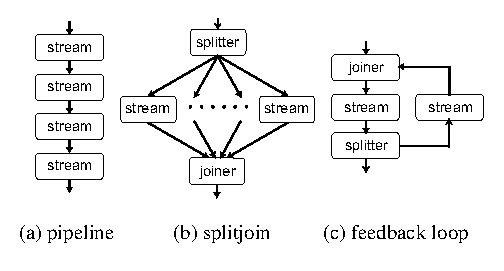
\includegraphics[scale=1, angle=0]{./constructs-eg.eps}
%}
% \vspace{-6pt}
% \nocaptionrule
 \caption{Hierarchical streams in StreamIt.}
 \label{fig:containers}
\end{center}
\end{figure}

\SubSection{Hierarchical Streams}
In StreamIt, the application developer focuses on the hierarchical
assembly of the stream graph and its communication topology, rather
than on the  explicit management of the data buffers between filters.
StreamIt provides three hierarchical structures for composing filters
into larger stream graphs (see Figure~\ref{fig:containers}).

\paragraph{Pipeline.}
The {\it pipeline} stream construct composes streams in sequence, with
the output of one connected to the input of the next.  An example of a
pipeline appears in Figure~\ref{fig:decoder-pipeline}. A pipeline is a
single input to single output stream. The decoding pipeline in the
figure consists of three streams. The first is a filter which zig-zag
unorders the input stream, and prepares the data for the inverse
quantization and DCT. The output of the filter is consumed by a stream
named {\tt IQ} which is a pipeline itself (not shown). This example
illustrates the hierarchical nature of stream composition in
StreamIt. The {\tt IQ} pipeline performs the inverse quantization, and
produces an output stream that is in turn consumed by another stream
which performs the inverse DCT. As in the case of a filter, pipelines
are also parameterizable.

\begin{figure*}[t]
  \begin{scriptsize}
    \begin{verbatim}
	int->int pipeline Decode()
	{ 
	  int Order[64] = {...};     // initialized as shown earlier
	  add ZigZagScan(64, Order);
	  add IQ();                  // inverse quantization
	  add IDCT(8, 8);            // inverse DCT (8x8 matrix)
	}
    \end{verbatim}
  \end{scriptsize}
  % \vspace{-3pt}
  \caption{Example MPEG decoder pipeline.}
  \label{fig:decoder-pipeline}
\end{figure*}

The {\tt add} keyword in StreamIt constructs the specified stream
using the input parameters. The {\tt add} statement may only appear in
non-filter streams.  In essence, filters are the leaves in the
hierarchical construction, and composite nodes in the stream graph
define the encapsulating containers. This allows for modular design
and development of large applications, thereby  promoting
collaboration, increasing code reuse, and simplifying debugging.

\paragraph{Split-Join.}
The {\it splitjoin} stream construct distributes data to a set of
parallel streams, which are then joined together in a roundrobin
fashion. In a splitjoin, the {\it splitter} performs the data
scattering, and the {\it joiner} performs the gathering. A splitter is
a specialized filter with a single input and multiple output
channels. On  every execution step, it can distribute its output to
any one of its children in either a {\it duplicate} or a {\it
roundrobin} manner. For the former, incoming data are replicated to
every sibling connected to the splitter. For the latter, data are
scattered in a roundrobin manner, with each item sent to exactly one
child stream, in order. The splitter type and the weights for
distributing data to child streams are declared as part of the syntax
(e.g., \texttt{split duplicate} or \texttt{split
roundrobin($w_1,\ldots,w_n$)}). The splitter counterpart is the
joiner. It is a specialized filter with  multiple input channels but
only one output channel. The joiner gathers data from its predecessors
in a roundrobin manner (declared as part of the syntax) to produce a
single output stream.

\begin{figure*}[t]
  \begin{scriptsize}
    \begin{verbatim}
	// N = macroblock size + motion vector data size;
	// W = picture width (resolution in pixels);
	// H = picture width (resolution in pixels);

	int->int splitjoin YCrCbDecoding(int N, int W, int H)
	{
	  // 4:2:0 chroma format
	  split roundrobin(4*N, 1*N, 1*N);

	  add LuminanceChannel  (W, H);
	  add ChrominanceChannel(W, H);
	  add ChrominanceChannel(W, H);

	  join roundrobin(1, 1, 1);  
	}
    \end{verbatim}
  \end{scriptsize}
  % \vspace{-3pt}
  \caption{Example MPEG decoder splitjoin.}
  \label{fig:decoder-sj}
\end{figure*}

The splitjoin stream is a convenient and natural way to represent
parallel computation. For example, when the decoder performs the
luminance and chrominance channel processing, the computation can
occur in parallel. In StreamIt, this is expressed as shown in
Figure~\ref{fig:decoder-sj}. The input stream contains the
macroblock data along with the parsed motion vectors. The data is
partitioned and passed to one of three decoding channels, with $4N$
items assigned to the first stream, $N$ items to the second, and $N$
items to the third. The three streams reconstruct the original
pictures with respect to the different color channels, and their
output is combined by the joiner to produce the final decoded picture.

\paragraph{Feedback Loop.}
StreamIt also provides a {\it feedback loop} construct for introducing
cycles in the graph. This stream construct is not used in the decoder,
but may be used in the MPEG encoder.

\paragraph{XXX: need to introduce messaging and talk about it.}
  \section{Graph Transformations}
\label{sec:transforms}

In this section we present a set of flexible transformations that can
be used to adjust the hierarchy and communication patterns of a
structured stream graph.  These transformations serve two purposes.
Firstly, they provide a means of deriving a canonical form: a program
representation that is insensitive to changes in the source code and
is easily analyzed by the compiler (for example, the hierarchical
ragged arrays of the partitioner).  Secondly, they serve as the
implementation mechanism by which the compiler arrives at an efficient
executable once it has analyzed the canonical form (for example, the
partitioner's traceback function).

Thus, we consider the transformations in pairs, each of which
represents a step in the opposite direction with respect to the
partitioner's representation.  After describing the transformations,
we describe the sequence in which they are employed when interfacing
to and from the partitioner.

\subsection{Vertical Cut Transformations}

The vertical cut transforms effect the distribution of parallel
streams across a hierarchy of splitjoin constructs (see
Figures~\ref{code:vert} and~\ref{ex:vert}).  The {\tt lowerChildren}
transform can factor any adjacent subset of a splitjoin's children
into a new splitjoin, which becomes a child of the original.  This is
a simple matter of re-arranging the weights in the splitters and
joiners.  It qualifies as a ``vertical cut'' transform because two
adjacent applications can divide a splitjoin with a vertical line.

The {\tt raiseChildren} transform will reverse the effect of any {\tt
lowerChildren} transform.  However, independent applications of this
transform are comparably rare: as detailed in the pseudocode, a child
can only be raised if its splitter type matches that of its parent,
and if the sums of its split and join weights match the corresponding
slots in the parent.

\subsection{Horizontal Cut Transformations}

The horizontal cut transforms are capable of transforming between a
splitjoin and a pipeline of splitjoins (see Figures~\ref{code:horiz}
and~\ref{ex:horiz}).  The {\tt addMatchingSyncPoints} transformation
inputs a rectangular splitjoin--one with pipeline children that have
equal lengths--and factors them into a sequence of splitjoins with
children that have unit length.  For the purpose of program analysis,
any splitjoin can be made rectangular by extending its shorter streams
with {\tt Identity} filters (a pre-defined node in StreamIt.)  Like an
hourglass, this transformation has the effect of squeezing a splitjoin
together at points of synchronization.

The {\tt removeMatchingSyncPoints} transformations directly implements
the inverse of {\tt addMatchingSyncPoints} via a simple re-arrangement
of weights.  Though very simple, this transformation can apply in
practice on interface boundaries where compound data streams are being
interleaved at a static rate.

A more aggressive transformation for synchronization removal is {\tt
removeStructuredSyncPoints} (see Figures~\ref{code:sync}
and~\ref{ex:sync}).  This algorithm removes not only synchronization
points with exactly matching weights, but it also expands any
join/split pair where the set of incoming and outgoing streams can be
partitioned such that no data item is passed between members of
different partitions during a steady-state execution.  The only
disadvantage of this transformation over {\tt
removeMatchingSyncPoints} is that it has the potential to introduce
non-adjacent joiners, which in the StreamIt compiler requires
additional processor resources.  However, like all transformations
described in this paper, the output of {\tt
removeStructuredSyncPoints} is still a structured graph (as the name
would suggest).

We have also implemented horizontal cut transforms for pipelines,
which consist simply of adding or removing a wrapper pipeline around a
sub-segment of the stream.  This is very straightforward (requiring no
change of weights or rates) so we omit the details here.

\subsection{Fusion and Fission Transformations}

Filter fusion describes a transform where several adjacent filters are
combined into one, while filter fission refers to the parallelization
of a filter via conversion to a splitjoin or pipeline.  These
transformations are at the heart of the load balancing partitioner
described in this paper.  A detailed description of fusion, fission,
and other intra-node transformations are described
in~\cite{streamit-asplos}; we restrict our attention to graph-level
transformations in this paper.

\subsection{Transforming to Partitioner's Representation}

To build the hierarchical arrays required by the partitioner, the
following transformations are applied, starting from the leaf nodes
and propagating upward through the stream:
\begin{itemize}

\item {\tt raiseChildren} and {\tt removeStructuredSyncPoints}
wherever possible.

\item {\tt removeMatchingSyncPoints} wherever possible.

\item Convert all non-rectangular splitjoins to rectangular ones by
extending their shorter child pipelines with Identity filters.

\item {\tt addMatchingSyncPoints} on all splitjoins.
\end{itemize}

The last step above will have the effect of replacing every splitjoin
with a pipeline of unit-length splitjoin constructs.  This pipeline is
exactly the representation that is sent to the partitioner; the width
of row {\tt y} is the width of the splitjoin at that location.  

\subsection{Transforming from Partitioner's Representation}

The traceback function is what calculates the sequence of
transformations needed to transform from the partitioner's
representation to the load-balanced set of partitions for program
execution.  In Figure~\ref{code:trace}, the points corresponding to a
vertical and horizontal cut are where traceback recurses after finding
the optimal {\tt xPivot} (for vertical cut) or {\tt yPivot} for
horizontal cut.  In our implementation, these cuts are recorded during
traceback, and then replayed on the stream graph at a later time.  The
only extra step to take is that synchronization must be removed before
any vertical cut is applied.

An example of the conversion to and from the partitioner's
representation appears in Figure~\ref{fig:trans}.

%% \section{Graph Transformations}
%% \label{sec:transforms}

%% We have developed a large suite of graph transformations that can be
%% used to adjust the hierarchy and communication patterns of a
%% structured stream graph.  These transformations--which include filter
%% fusion, filter fission, horizontal cuts, vertical cuts, and aggressive
%% synchronization removal--serve two distinct purposes.  Firstly, they
%% provide a means of deriving a canonical form: a program representation
%% that is insensitive to changes in the source code and is easily
%% analyzed by the compiler (for example, the hierarchical ragged arrays
%% of the partitioner).  Secondly, they serve as the implementation
%% mechanism by which the compiler arrives at an efficient executable
%% once it has analyzed the canonical form (for example, the
%% partitioner's traceback function).  In our final paper, we will
%% describe these transformations in detail, as well as their role in the
%% structured partitioning algorithm.

%  structures
-------------------------------------------------------------------------
container s:
  s.height       : returns height of region
  s.width[i]     : returns width of i'th row
  s.get(i, j)    : returns the (i,j)'th child

globals
-------------------------------------------------------------------------
// A_s[x1][x2][y1][y2][n] holds minimum cost of assigning children 
// (x1..x2, y1..y2) of stream s to n tiles
forall s in graph:  int[][][][][] A_s;

// do partitioning of stream s on n tiles and return mapping from node
// to partition number
stream->int toplevel(stream s, int n)
-------------------------------------------------------------------------
setup(n)
cost = getCost(s, n)
// if desired, eliminate extra partitions that aren't contributing to
// the cost
while (n>1 && getCost(s, n-1)==cost)
  n--
endwhile
traceback(s, empty-map, 0, n)
return map

// setup for n partitions
void setup(int n) 
-------------------------------------------------------------------------
(pad all splitjoins so that each parallel stream is same length)
(add maximal synchronization to all splitjoins)
(consider feedbackloops as a 2-way splitjoin, each child of which is a
 2-element pipeline (to prevent fusing with loop/body separately)
(eliminate all splitjoins in pipelines in favor of rectangular pipelines)

forall s in graph
  A_s = new int[s.length()][s.length()][s.width()][s.width()][n]
  forall (x1,x2,y1,y2,n) \in A_s
    A[x1][x2][y1][y2][n] = -1

// return minimal cost for allocating <n> partitions to children
int getCost(stream s, int n)
-------------------------------------------------------------------------
// see if we will need a joiner
if (n>1 && needsJoiner(s)) 
  n--
if (s is Node)
  return getNodeCost(s, n)
if (s is Container)
  int maxWidth = max(s.width[0], ..., s.width[s.height]);
  return getContCost(s, 0, maxWidth-1, 0, s.height-1, n)
endif

// returns whether or not stream <s> needs a joiner if it is spread
// across multiple tiles
boolean needsJoiner (stream s)
-------------------------------------------------------------------------
par = s.parent()
if (par==null)
  // if have no parent, then need a joiner
  return true
else if (par.width()>1)
  // if par has multiple streams, it will have joiner instead
  return false;
else if (par.parent()==null && s!=par.get(0, par.length()-1))
  // if we're in middle of toplevel stream, then need joiner
  return true
else
  // otherwise we're guaranteed by lifter that par.parent().width>1,
  // so there will be a joiner there and we don't need one for s
  return false
end if

  \section{Results}
\label{chpt:results}

This section presents results of creating schedules using
techniques described in Sections \ref{chpt:hierarchical} and
\ref{chpt:phased}.

Section \ref{sec:results:apps} presents the applications used for
testing.  Section \ref{sec:results:results} presents the results and
analysis.

\subsection{Applications}
\label{sec:results:apps}

Our benchmark suite contains 17 applications. Out of those
applications, 15 represent useful practical computation taken from
real-life applications, while two were chosen to highlight the
effectiveness of phased scheduling.

SJPeek1024 and SJPeek31 are synthetic benchmarks, designed to
highlight strengths of phased schedules. SJPeek1024 requires an
initialization schedule which benefits from finer granularity of
minimum latency schedule. SJPeek31 contains a push/pop mismatch
which causes a combinatorial blow-up using SAS.

Nine test applications (BitonicSort, FFT, FilterBank, FIR, Radio,
GSM, 3GPP, Radar and Vocoder) are applications used in
\cite{Gordo02}. BitonicSort performs a 32 element bitonic sort.
FFT performs a 64-element FFT, FilterBank is an 8 channel filter
bank.  FIR is a 64-tap FIR application. Radio is an FM radio
decoder with an equalizer.  3GPP is a 3GPP Radio Access Protocol
application. Radar is a radar array front-end application. Vocoder
is a 28 channel Vocoder.

Two test applications (QMF and CD-DAT) are applications used in
another publication on scheduling streaming applications
(\cite{murthy99buffer}). QMF is a filter bank application. CD-DAT
is a sample rate conversion application. The code inside of the
{\filters} has not been implemented. QMF application is a
qmf12\_3d.  It was slightly modified to account for {\StreamIt}
{\splitters} and {\joiners} not allowing any computation. The
high-pass and low-pass filtering in the {\splitters} has been
moved to just after data has been separated into two channels. The
re-combining of data in the {\joiners} has been moved to a
{\filter} just after the {\joiners}. The low and high pass filters
have also been given a peek amount of 16 so they can perform their
function in the way intended in {\StreamIt}.
 CD-DAT is exactly the same application as
that described in \cite{murthy99buffer}.

The remaining 4 applications were chosen from our sample
applications used for testing the StreamIt compiler. HDTV performs
a HDTV signal decoding/encoding. CFAR implements PCA Constant
False Alarm Rate detection. Block Matrix Mult performs a blocked
matrix multiplication application - it multiplies a 12x12 matrix
by a 9x12 matrix in blocks of 3x3 submatrices. Trellis performs
trellis encoding/decoding.

\begin{comment}

\subsection{Methodology}
\label{sec:results:methodology}

The following data has been collected: number of nodes, number of
node executions per steady state, schedule size and buffer size
for pseudo single appearance and minimal latency schedules.

\subsubsection{Schedule Compression}

\end{comment}

\begin{comment}
\subsubsection{Sinks}

Any application in {\StreamIt} must receive its data from outside,
and its data must be sent to outside. {\filters} that receive and
send data to outside are called sinks and sources. In particular,
sinks have the property of having $u_f = 0$ while sources have
$e_f = o_f = 0$. Sinks are problematic for minimal latency
scheduling, because they do not produce any data. Thus any
schedule of a sink operator is a minimal latency schedule. This
leads to the minimal latency schedule of the outer-most
{\pipeline} becoming a single appearance schedule, thus destroying
some of the benefit of using phased scheduling. The technique
used for scheduling {\pipeline} sinks has been discussed in
\cite{karczma-thesis}.

This problem has been alleviated by detecting sinks at the end of
a {\pipeline} and scheduling them in a unique way. Namely, a simple
attempt is made to minimize the amount of storage necessary to
store the phases of the {\pipeline}.

Let the amount of storage necessary to store one data item in
{\Input} {\Channel} to the sink be $x$, the amount of storage necessary
to store a phase be $y$, the sink consume $a$ data per steady
state execution of its parent {\pipeline} and $b$ be the number of
phases of the parent pipeline, then we have that amount of storage
necessary to store the phases and the buffer is
$$ {ax \over b} + by $$ We want to minimize this amount, with $b$
being the variable. We take a derrivative of the above expression,
set it to zero and solve:

\begin{displaymath}
\begin{array}{rcl}
-{ax \over b^2} + y & = & 0 \\
yb^2 & = & ax \\
b & = & \sqrt{ax \over y}
\end{array}
\end{displaymath}

For simplicity, we set $x = y = 1$, thus obtaining that $b =
\sqrt{a}$.

Now, for every phase of the parent {\pipeline} of the sink, the sink
is executed $\sqrt{a}$ times on the first step of scheduling a
phase of the {\pipeline}.
\end{comment}

\subsection{Results}
\label{sec:results:results}

\begin{figure}[t]
\psfig{figure=buffer-graph.eps,width=3.35in}
\caption{Buffer sizes.}
\end{figure}

\begin{figure}[t]
\psfig{figure=code-graph.eps,width=3.35in}
\caption{Code sizes.}
\end{figure}

\begin{figure}[t]
\psfig{figure=total-size-graph.eps,width=3.35in}
\caption{Sum of code size and buffer size.}
\end{figure}

\begin{table*} \centering \small
\begin{tabular}{|c|c|c|c|c|c|c|}
\hline benchmark & \parbox{0.5in}{\centering number of nodes} & \parbox{0.5in}{\centering number of node executions} & \multicolumn{2}{c|}{pseudo single appearance} & \multicolumn{2}{c|}{minimal latency} \\
\cline{4-7} & & & \parbox{0.5in}{\centering schedule size} & \parbox{0.5in}{\centering buffer size} & \parbox{0.5in}{\centering schedule size} & \parbox{0.5in}{\centering buffer size} \\
\hline SJPeek31 & 6 & 12063 & 8 & 19964 & 24 & 874 \\
\hline HDTV & 170 & 390038 & 230 & 550692 & 1190 & 28300 \\
\hline CD-DAT & 6 & 612 & 6 & 1021 & 64 & 72 \\
\hline CFAR & 4 & 193 & 7 & 193 & 9 & 129 \\
\hline SJPeek1024 & 6 & 3081 & 8 & 7168 & 13 & 4864 \\
\hline Block Matrix Mult & 43 & 1956 & 48 & 4212 & 56 & 3132 \\
\hline Vocoder & 117 & 415 & 156 & 1285 & 205 & 1094 \\
\hline Radar & 68 & 161 & 68 & 332 & 68 & 332 \\
\hline BitonicSort & 370 & 468 & 370 & 2112 & 370 & 2112 \\
\hline 3GPP & 94 & 356 & 104 & 986 & 108 & 970 \\
\hline Trellis & 14 & 301 & 14 & 538 & 17 & 499 \\
\hline FIRfine & 132 & 152 & 132 & 1560 & 132 & 1560 \\
\hline FilterBank & 53 & 312 & 95 & 2063 & 116 & 1991 \\
\hline QMF & 65 & 184 & 85 & 1225 & 85 & 1225 \\
\hline Radio & 30 & 43 & 35 & 1351 & 35 & 1351 \\
\hline FFT & 26 & 448 & 26 & 3584 & 26 & 3584 \\
\hline GSM & 47 & 3356 & - & - & 64 & 3900 \\
\hline
\end{tabular}
\caption{Results of running pseudo single appearance and minimal
latency scheduling algorithms on various applications.}
\label{tbl:results}
\end{table*}

\begin{comment}
\begin{figure}
\centering \psfig{figure=kz-1.eps,width=6in} \caption[Buffer
storage space savings of Phased Minimal Latency schedule vs.
Hierarchical schedule.]{Buffer storage space savings of Phased
Minimal Latency schedule vs. Hierarchical schedule. All data in
all {\Channels} is assume to consume same amount of space.}
\end{figure}

\begin{figure}
\centering \psfig{figure=kz-2.eps,width=6in} \caption[Storage
usage comparison]{Storage usage for compressed Minimal Latency
Phased schedule vs. Hierarchical schedule. Left bars are for
Hierarchical schedules. Numbers are normalized to total storage
required by Hierarchical schedule. Each entry in every schedule
and data items in all {\Channels} are assumed to consume same
amount of space.}
\end{figure}
\end{comment}

Table \ref{tbl:results} presents buffer and schedule sizes
necessary to execute various applications using the algorithms
developed in this thesis.

The GSM application cannot be scheduled using pseudo
single-appearance algorithm, because it has a loop which is too
tight for execution under the SAS.

Several applications show a very large improvement in buffer size
necessary for execution.  Namely, CD-DAT decreases from 1021 to
72, a 93\% improvement. \cite{murthy99buffer} reports a buffer
size of 226 after applying buffer merging techniques. Our
improvement is due to reducing the combinatorial growth of the
buffers using phased scheduling.

Our synthetic benchmarks decrease from 7168 to 4864 and from 19964
to 12063, a 32\% and 40\% improvements. The first improvement is
due to creating fine grained phases which allow the initialization
schedule to transfer smaller amount of data and allow the children
of a {\splitjoin} to drain their data before the {\splitter}
provides them with more. This improvement is only created in
presence of peeking. The second improvement is due to reducing
combinatorial growth and due to finer grained schedules to deal
with peeking.

Other applications show no or little improvement in buffer
requirements. As expected, no application requires more buffer
space.

  \section{Non-Hierarchical  Transformations}

\section{Non-Hierarchical Graph Transformations}

\subsection{Vertical SplitJoin Fission}

Can pull out a node from a splitjoin.

\subsection{}

\subsection{Unstructured Syncronization Removal}


\section{Non-Hierarchical Cost Functions}

\subsubsection{Layout}

\subsubsection{Communication}






  \begin{figure}[t]
    \psfig{figure=algorithm4.eps,width=3.5in}
    \caption{Refactoring hierarchical splitjoin children.}
  \end{figure}
  
  \begin{figure}[t]
    \psfig{figure=algorithm5.eps,width=3.5in}
    \caption{Adding and removing splitjoin synchronization.}
  \end{figure}
  
  \begin{figure}[t]
    \psfig{figure=algorithm6.eps,width=3.5in}
    \caption{Aggressive synchronization removal.}
  \end{figure}
  
  \clearpage
  \begin{figure*}[t]
    \begin{tabular}{ll}
    \psfig{figure=algorithm.eps,width=3.5in}
    &
    \psfig{figure=algorithm2.eps,width=3.5in}
    \end{tabular}
    \caption{Search phase of the partitioning algorithm.  The traceback phase appears in the appendix.
      \protect\label{code:partition}}
  \end{figure*}

  \section*{Appendix}
  \clearpage
  \begin{figure}[t]
    \psfig{figure=algorithm3.eps,width=3.5in}
  \end{figure}
  
  % Bibliography -- whee!
  \begin{small}
    \bibliographystyle{abbrv}
    \bibliography{references}
  \end{small}
  
\end{document}